\section{Background}

\begin{frame}{Information Flow and Access Control}
	Many systems control access to information with \textbf{access control} mechanisms, which place restrictions based on the \textit{permissions} of a user or of calling code but which cannot restrict how that information \textit{propagates} once released \cite{ifbackground:sabelfeld}.
	
	\textbf{Information flow} mechanisms instead control access by enforcing that some \textit{policy} on the data is upheld.
	
	In short, access control puts controls on the \textit{calling code}, where information flow puts controls on the \textit{data}.
\end{frame}

\begin{frame}{Information Flow Basics}
	Information Flow considers \textit{confidentiality states}. Flow \textit{policies} formalise how information may move between states.
	
	One common representation is the Bell-LaPadula Lattice model used in Mandatory Access Control. An alternative is representing policies using logical predicates.
	
	\begin{figure}
		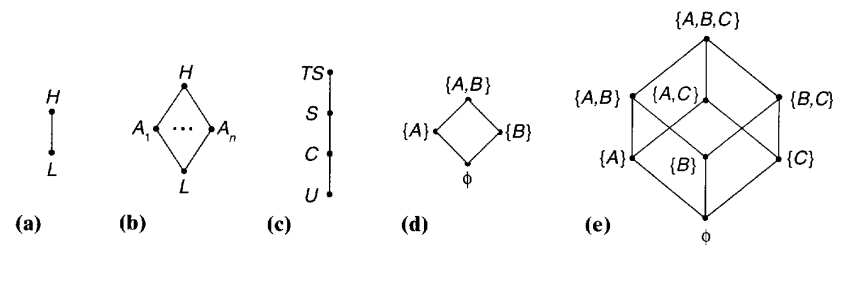
\includegraphics[scale=0.45]{content/images/lattice_examples.png}
		\caption{Example Lattice Model policies \cite{ifbackground:sandhu}}
	\end{figure}
	
\end{frame}

\begin{frame}{Noninterference}
	
	Information Flow theory can provide provable confidentiality:
	\begin{block}{Noninterference}
		A program is noninterfering if any two different executions which differ only in their high confidentiality inputs are indistinguishable to an attacker. \cite{ifbackground:goguen}
	\end{block}
	\begin{itemize}
		\item Proving non-interference (in the general case) is undecidable
			\begin{itemize}
				\item The halting problem can be reduced to it
			\end{itemize}
		\item Many useful programs are inherently interfering
			\begin{itemize}
				\item A password checker's output clearly depends on the password
			\end{itemize}
	\end{itemize}
\end{frame}

%\begin{frame}{Noninterference - Is It Practical?}
%	Problems with proving noninterference:
%	
%	\begin{enumerate}
%		\item Proving non-interference (in the general case) is undecidable
%			\begin{itemize}
%				\item The halting problem can be reduced to it -- consider: \newline \texttt{\textbf{if} S() halts \textbf{then} h := 1 \textbf{else} h := 0} \cite{ifbackground:denninghalting}
%				\item \textit{Most real systems prove a simplified case using type checking}
%			\end{itemize}
%		\item Many useful programs are inherently interfering
%			\begin{itemize}
%				\item A password checker's output clearly depends on the password
%				\item \textit{Most real systems allow for `selective declassification'}
%			\end{itemize}
%		\item Noninterference does not model covert channels
%			\begin{itemize}
%				\item \textit{Some systems secure against specific potential covert channels}
%				\item There is no way to prove that no covert channels exist
%			\end{itemize}
%	\end{enumerate}
%\end{frame}

\begin{frame}{Enforcement: Static or Dynamic?}
	Controls be enforced at compile-time or at run-time.
	
	\textbf{Static} information flow controls produce no run-time overhead, and can much more easily track `implicit flows'.
	
	\textbf{Dynamic} information flow controls include some overhead and cannot track implicit flows, but can be more flexible and can represent a wider range of policies.
	
	Most solutions use static or `mostly static' approaches.
\end{frame}

\begin{frame}{Information Flow and Integrity}
	Information flow is usually talked about with respect to confidentiality, but it can also be applied to integrity.
	
	For \textbf{Confidentiality}:\newline Track the flow of high confidentiality (`secret') outputs.
	
	For \textbf{Integrity}:\newline Track the flow of low integrity (`tainted') inputs.
\end{frame}